\section{Requirements and Design Choices}
The functional requirements the package should meet, and how these are met will be described in this section. Fundamentally the package should support the computation of the features described in \ref{chapter:03} however there are several layers to achieving this, including the following:

\begin{itemize}
    \item Saving and loading of Location Samples on the device
    \item Computing intermediate features from Location Samples
    \item Saving and loading Stops and Moves on the device
    \item Computing the features
\end{itemize}

Saving and loading of Location Samples is necessary in order to not lose data. When an application tracks location data for a pro-longed period of time, i.e. a whole day, it will risky to keep all the collected data in RAM, since all data is lost if the app is killed by accident either by the OS or the user. For computing the Routine Index it was necessary to store historical data, in order to compare days. Intermediate features made this possible by bringing the storage requirements down significantly, compared to storing raw Location Samples on the device. A normal day of tracking could result in up to 18,000 Location Samples which is quite a lot of data considering the algorithms need up to 28 days of data. In addition, converting a dataset of raw Location Samples into Stops also made the computation for finding Places, and thereby many of the mobility features, much cheaper. Lastly, computing mobility features should be possible at any time, even if the day is incomplete. This has been taken care of by the definitions made in Chapter \ref{chapter:03} by redefining features such that they can be evaluated on incomplete days.

\subsection{Storing and Loading}
Since historical data is a major factor in computing the features, it was decided to include an easy way for the programmer to store and load Location Samples. To store objects in an Object Oriented Language serialization \footnote{\url{\footnote{\url{https://www.martinfowler.com/eaaCatalog/serializedLOB.html}}}} can be used, which is act of transforming an object into a graph of smaller objects in a data format which can be written to a file. A serialized object, in contrast to an entity stored in database is already pre-assembled. In a database this assembly happens via joins since the object is spread over multiple tables. The database may store the object more efficiently, but it does not come pre-assembled. This is analogous to how a set of Legos blocks comes in a box rather than already being pre-assembled. While traditional databases usually scale better than serialization they come with an overhead cost of being time consuming to set up properly. For this reason serialization was chosen in favor of databases,  since the project was small. In addition it is also very easy to import serialized objects into other programming languages, such as Python for data analysis. 

\subsection{Data Format}
The data format used was JSON (JavaScript Object Notation) which is a very common, human-readable data format that uses key-value pairs to store data. A JSON object can be stored in a database, or it can be transformed to a string in order to be stored. It was chosen to simply transform JSON objects to a string and write them to a local file, rather than storing the information in a database on the phone. 
JSON supports a limited number of data types, such as strings, numbers, booleans, arrays, objects and null values. This means that in order to translate a Dart object to JSON, all of its fields must be serializable. An example of where this quickly becomes a problem, is with objects such as DateTime objects, since they are not supported by JSON - however a DateTime can be transformed to a number, which is milliseconds since epoch, or to an ISO standard date string. The approach is therefore to look at all the fields of the object that is to be serialized, and ensure that types of these fields all support some form of serialization. If they do not, it must be implemented.

\subsection{Computing Features}
Data collection will be done by the programmer
Should be saved regularily
Historical data is loaded
Compute places more accurately using historical data
If prior are selected then compute old contexts
Add these contexts to to todays contect such that the routine index may be calculated


\begin{figure}
    \centering
    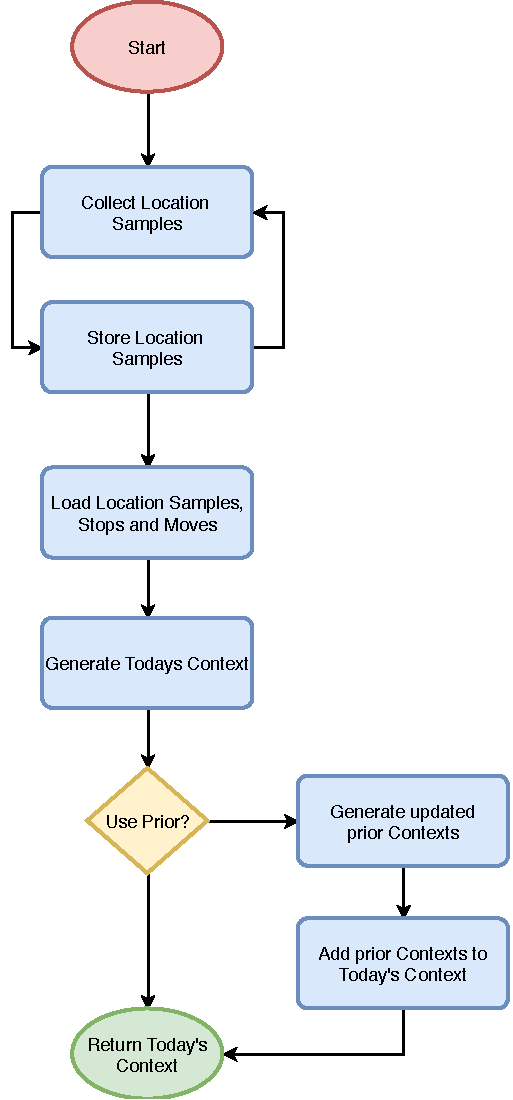
\includegraphics[width=0.5\textwidth]{images/diagrams/api-flowchart.pdf}
    \caption{The flowchart for computing mobility features using historical data}
    \label{fig:my_label}
\end{figure}


